\chapter{व्यायाम और शरीर की ऊर्जा-ज़रूरतें}\label{ch:g10:exercise-and-energy}

प्रयोगशाला की साइकिल पर बैठी एक साइकिल-सवार ऐसे ब्रेक के ख़िलाफ़ पैडल
मारती है जो उसकी शक्ति नापता है: \qty{100}{W}, फिर \qty{150}{W}, फिर
\qty{200}{W}। उसके चेहरे पर लगा मुखौटा हर साँस एक विश्लेषक तक भेजता है।
पर्दे पर के अंक ब्रेक के साथ-साथ चढ़ते हैं: वह जितना अधिक यांत्रिक कार्य
देती है, उतनी ही अधिक ऑक्सीजन खपाती है और उतनी ही अधिक कार्बन डाइऑक्साइड
बाहर छोड़ती है। उसकी पेशियाँ \cref{ch:g10:cell-metabolism} वाला श्वसन पूरे
ज़ोर से चला रही हैं, और विश्लेषक उसी का बही-खाता पढ़ रहा है। यह अध्याय
व्यायाम की ऊर्जा का पीछा उस भोजन से करता है जो उसे देता है, उस ऑक्सीजन
तक जो उसे छोड़ती है।

\section{ऊर्जा भीतर, कार्य बाहर}

\begin{definition}[ऊर्जा व्यय]\label{def:g10:exercise-and-energy:expenditure}
शरीर का \emph{ऊर्जा व्यय}\index{ऊर्जा व्यय}, जूल में, वह कुल ऊर्जा है जो
उसकी \omterm{def:g10:cells-common-unit:cell}{कोशिकाएँ} किसी दिए हुए समय में कार्बनिक अणुओं से छोड़ती हैं। समय से
भाग देने पर वह \emph{उपापचयी शक्ति} बन जाती है, वाट में। विश्राम में कोई
वयस्क लगभग \qty{80}{W} ख़र्च करता है --- यानी दिन भर में क़रीब
\qty{7000}{kJ} --- ताकि हृदय धड़कता रहे, मस्तिष्क काम करता रहे, ताप
\qty{37}{\celsius} पर बना रहे और \omterm{def:g10:cells-common-unit:cell}{कोशिकाएँ} जीवित रहें; यही
\emph{आधारी \omterm{def:g10:cell-metabolism:metabolism}{उपापचय}} है। हर गतिविधि उसमें और जोड़ती है।
\end{definition}

\begin{proposition}[ऊर्जा जाती कहाँ है]\label{prop:g10:exercise-and-energy:efficiency}
काम करती पेशी अपनी छोड़ी हुई ऊर्जा का केवल लगभग एक-चौथाई ही यांत्रिक
कार्य में बदलती है; बाक़ी तीन-चौथाई ऊष्मा बनकर निकल जाता है। इसलिए
$P$ यांत्रिक शक्ति देने पर शरीर को विश्राम से ऊपर लगभग $4P$ उपापचयी
शक्ति ख़र्च करनी पड़ती है: पैडल पर \qty{100}{W} देती साइकिल-सवार अपनी
पेशियों में क़रीब \qty{400}{W} ख़र्च कर रही है, और उसके शरीर को
\qty{300}{W} ऊष्मा से पीछा छुड़ाना पड़ता है --- ज़्यादातर पसीने से।
\end{proposition}
\admitted

\begin{example}[रोज़ के बजट]\label{ex:g10:exercise-and-energy:budgets}
कक्षा में बैठा, स्कूल तक चलकर जाता और सोता विद्यार्थी दिन भर में लगभग
\qty{9000}{kJ} ख़र्च करता है; फ़ुटबॉल का एक घंटा क़रीब \qty{2500}{kJ} और
जोड़ देता है; और पीठ पर बोझ लिए पहाड़ों में बिताया दिन कुल मिलाकर
\qty{15000}{kJ}। किसी दौड़ के पहाड़ी चरण पर साइकिल-सवार \qty{25000}{kJ}
ख़र्च करती है, और दिन भर में उतना खा भी नहीं पाती। यह ऊर्जा भोजन से आती
है (\cref{ch:g10:chemistry-of-life}): \omterm{def:g10:chemistry-of-life:families}{कार्बोहाइड्रेट} या \omterm{def:g10:chemistry-of-life:families}{प्रोटीन} के प्रति
ग्राम \qty{17}{kJ}, और \omterm{def:g10:chemistry-of-life:families}{लिपिड} के प्रति ग्राम \qty{38}{kJ}।
\end{example}

\section{ऑक्सीजन की खपत ऊर्जा व्यय नापती है}

\begin{proposition}[ऑक्सीजन तुल्यांक]\label{prop:g10:exercise-and-energy:oxygen}
चूँकि व्यायाम की ऊर्जा \omterm{prop:g10:cell-metabolism:respiration}{कोशिकीय श्वसन} से छूटती है, जो ऑक्सीजन खपाता है,
इसलिए शरीर की ऑक्सीजन-खपत ही उसका \omterm{def:g10:exercise-and-energy:expenditure}{ऊर्जा व्यय} नाप देती है: खपी हुई हर लीटर
ऑक्सीजन लगभग \qty{20}{kJ} छूटने के बराबर है, चाहे ग्लूकोज़ और \omterm{def:g10:chemistry-of-life:families}{लिपिड} का
मिश्रण जो भी जलाया जा रहा हो। विश्राम में कोई व्यक्ति प्रति मिनट लगभग
\qty{0.25}{L} ऑक्सीजन खपाता है; और व्यायाम के दौरान खपत दी जा रही शक्ति
के अनुपात में बढ़ती है, अपनी एक निजी छत तक।
\end{proposition}
\begin{proof}[साक्ष्य]
\cref{ch:g10:cell-metabolism} का श्वसन समीकरण \qty{6}{mol} ऑक्सीजन के
लिए \qty{2870}{kJ} देता है, यानी प्रति मोल \qty{478}{kJ}, और एक मोल गैस
लगभग \qty{24}{L} घेरती है: यानी प्रति लीटर \qty{20}{kJ}। \omterm{def:g10:chemistry-of-life:families}{लिपिड} के लिए यह
आँकड़ा \qty{19.6}{kJ/L} है और \omterm{def:g10:chemistry-of-life:families}{कार्बोहाइड्रेट} के लिए \qty{21.1}{kJ/L},
इसलिए मिश्रण से शायद ही कोई फ़र्क़ पड़ता है। बंद कक्षों में की गई
मापें, जहाँ किसी व्यक्ति की छोड़ी हुई ऊष्मा सीधे बटोरी जाती है, ऑक्सीजन
वाले आँकड़े से कुछ प्रतिशत के भीतर मेल खाती हैं।
\end{proof}

\begin{omfigure}
\begin{tikzpicture}
\begin{axis}[
  width=0.86\linewidth, height=5.8cm,
  axis x line=bottom, axis y line=left,
  xmin=0, xmax=320, ymin=0, ymax=4.2,
  xlabel={यांत्रिक शक्ति (\unit{W})}, ylabel={खपी $\mathrm{O_2}$ (\unit{L/min})},
  xlabel style={font=\small, at={(axis description cs:0.5,-0.12)}, anchor=north},
  ylabel style={font=\small},
  tick label style={font=\small},
  xtick={0,50,100,150,200,250,300}, ytick={0,1,2,3,4},
  clip=false,
]
\addplot[thick, omThm, mark=*, mark size=1.6pt] coordinates
  {(0,0.3) (50,0.9) (100,1.5) (150,2.1) (200,2.7) (250,3.2) (300,3.3)};
\draw[dashed, gray] (axis cs:0,3.3) -- (axis cs:320,3.3);
\node[font=\small, anchor=south east] at (axis cs:318,3.32) {अधिकतम $\dot V\!\mathrm{O_2}$};
\node[font=\small, anchor=south west, align=left] at (axis cs:40,3.42) {ढाल: हर वाट के लिए प्रति मिनट\\ $\mathrm{O_2}$ के \qty{12}{mL}};
\end{axis}
\end{tikzpicture}

{\small बढ़ती शक्ति पर पैडल मारते किसी व्यक्ति की ऑक्सीजन-खपत। बढ़त रैखिक
है --- प्रति वाट प्रति मिनट लगभग \qty{12}{mL} ऑक्सीजन --- जब तक खपत अपनी
छत, यानी उस व्यक्ति की अधिकतम $\dot V\!\mathrm{O_2}$, तक न पहुँच जाए;
उसके आगे की अतिरिक्त शक्ति बिना ऑक्सीजन के जुटाई जाती है और लंबे समय तक
टिक नहीं सकती।}
\end{omfigure}

\begin{definition}[अधिकतम ऑक्सीजन खपत]\label{def:g10:exercise-and-energy:vo2max}
\emph{अधिकतम ऑक्सीजन खपत}\index{अधिकतम ऑक्सीजन खपत}, जिसे
$\dot V\!\mathrm{O_2}$ की अधिकतम मान कहा जाता है, वह सबसे ऊँची दर है जिस
पर किसी व्यक्ति का शरीर ऑक्सीजन ले और इस्तेमाल कर सकता है, लीटर प्रति
मिनट में --- या, अलग-अलग आकार के लोगों की तुलना के लिए, प्रति किलोग्राम
शरीर-द्रव्यमान पर मिलीलीटर प्रति मिनट में। वही वह सबसे ऊँची शक्ति तय करती
है जो अकेले श्वसन से टिकाई जा सके। ठेठ मान: गतिहीन वयस्क में प्रति
किलोग्राम \qty{35}{mL/min}, प्रशिक्षित विद्यार्थी में \num{50}, और
सहनशक्ति के किसी चैंपियन खिलाड़ी में \num{80} या उससे भी अधिक।
\end{definition}

\begin{example}[वक्र पढ़ना]\label{ex:g10:exercise-and-energy:reading}
चित्र में \qty{100}{W} पर पैडल मारने का दाम प्रति मिनट \qty{1.5}{L/min}
ऑक्सीजन है: यानी प्रति मिनट $1.5 \times 20 = \qty{30}{kJ}$, यानी
\qty{500}{W} उपापचयी शक्ति --- कार्य के \qty{100}{W} और उनके ऊपर ऊष्मा
तथा विश्राम की ज़रूरतों के \qty{400}{W}, ठीक
\cref{prop:g10:exercise-and-energy:efficiency} के अनुरूप।
\qty{66}{kg} के व्यक्ति के लिए \qty{3.3}{L/min} की छत प्रति किलोग्राम
\qty{50}{mL/min} बनती है।
\end{example}

\begin{omfigure}
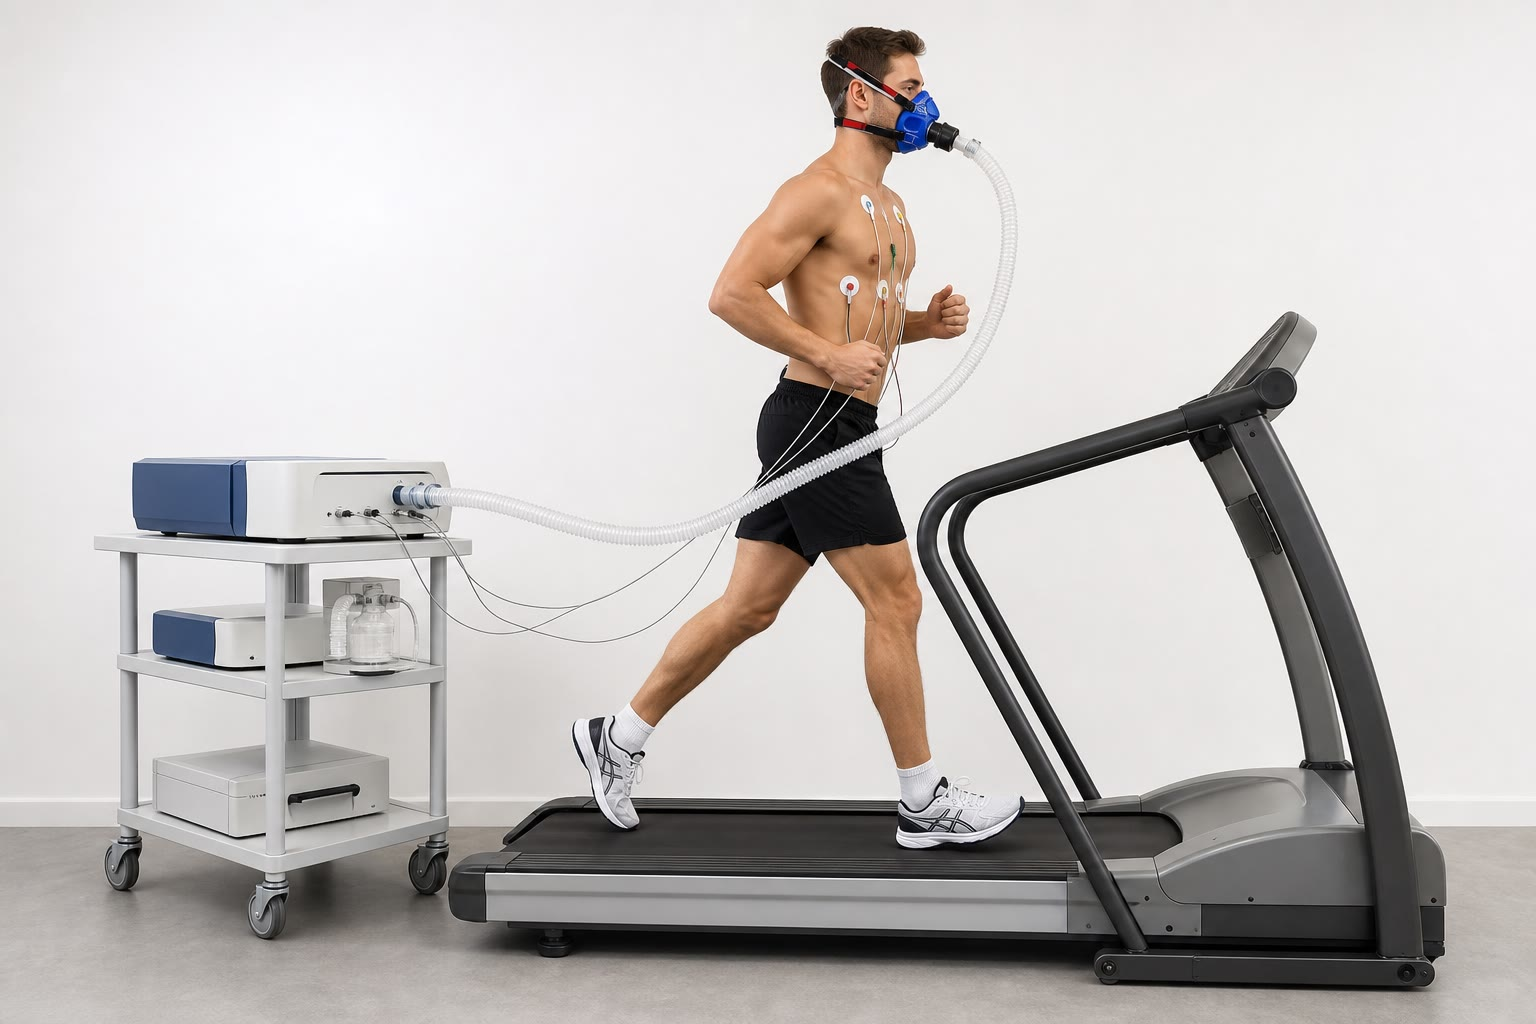
\includegraphics[width=0.62\linewidth]{images/book2/ai/g10-exercise-treadmill-mask.jpg}

{\small व्यायाम के दौरान ऑक्सीजन-खपत नापना: हर साँस मुखौटे से होकर एक
गैस-विश्लेषक तक जाती है, जो मिनट-दर-मिनट ली गई ऑक्सीजन और छोड़ी गई कार्बन
डाइऑक्साइड दर्ज करता है, जबकि ट्रेडमिल शक्ति तय करता है।}
\end{omfigure}

\section{पेशी के ईंधन}

\begin{proposition}[ATP के तीन स्रोत]\label{prop:g10:exercise-and-energy:fuels}
पेशी के संकुचन का दाम ATP में चुकाया जाता है, और \omterm{def:g10:cells-common-unit:cell}{कोशिका} उसे केवल कुछ
सेकंड भर रखती है। उसे तीन रास्तों से नया किया जाता है, और हर रास्ते की
अपनी रफ़्तार तथा अपनी क्षमता है:
\begin{itemize}
  \item पेशी में किसी फ़ॉस्फ़ेट यौगिक का एक छोटा भंडार, जो ATP तुरंत
        दोबारा बना देता है पर लगभग दस सेकंड ही चलता है --- यानी
        फ़र्राटा दौड़;
  \item \omterm{def:g10:cells-common-unit:cell}{कोशिकाद्रव्य} में ग्लूकोज़ का लैक्टिक \omterm{def:g10:cell-metabolism:fermentation}{किण्वन}, जो तेज़ पर फ़िज़ूलख़र्च
        है, पूरे ज़ोर की कोशिश को एक से दो मिनट तक टिकाता है और लैक्टिक
        अम्ल बनाता है;
  \item \omterm{def:g10:cells-common-unit:organelle}{सूत्रकणिकाओं} में \omterm{prop:g10:cell-metabolism:respiration}{कोशिकीय श्वसन}, जो पूरी दर तक पहुँचने में धीमा है
        पर अवधि में लगभग असीम, और जो रक्त का ग्लूकोज़, पेशी का \omterm{def:g10:exercise-and-energy:glycogen}{ग्लाइकोजन}
        तथा शरीर की चर्बी के वसा-अम्ल जलाता है।
\end{itemize}
इनमें से हर एक का हिस्सा व्यायाम की तीव्रता और अवधि पर निर्भर करता है।
\end{proposition}
\admitted

\begin{omfigure}
\begin{tikzpicture}
\begin{axis}[
  ybar stacked, bar width=18pt,
  width=0.86\linewidth, height=5.6cm,
  axis x line=bottom, axis y line=left,
  ymin=0, ymax=100, ylabel={ऊर्जा में हिस्सा (\%)}, ylabel style={font=\small},
  symbolic x coords={10 s, 1 min, 4 min, 30 min, 2 h},
  xtick=data, tick label style={font=\small},
  xlabel={पूरे ज़ोर की कोशिश की अवधि},
  xlabel style={font=\small, at={(axis description cs:0.5,-0.12)}, anchor=north},
  enlarge x limits=0.15,
  legend style={at={(0.5,-0.3)}, anchor=north, legend columns=3,
                font=\small, draw=none},
]
\addplot[fill=omThm!50, draw=omThm] coordinates {(10 s,85) (1 min,25) (4 min,8) (30 min,2) (2 h,1)};
\addplot[fill=omProp!50, draw=omProp] coordinates {(10 s,12) (1 min,50) (4 min,32) (30 min,8) (2 h,2)};
\addplot[fill=omDef!50, draw=omDef] coordinates {(10 s,3) (1 min,25) (4 min,60) (30 min,90) (2 h,97)};
\legend{फ़ॉस्फ़ेट भंडार, लैक्टिक किण्वन, श्वसन}
\end{axis}
\end{tikzpicture}

{\small दी हुई अवधि की पूरे ज़ोर वाली कोशिश में ATP के तीनों स्रोतों का
अनुमानित हिस्सा। 100 मीटर की फ़र्राटा दौड़ फ़ॉस्फ़ेट भंडार पर चलती है;
400 मीटर की दौड़ बड़े हिस्से में \omterm{def:g10:cell-metabolism:fermentation}{किण्वन} पर; और कुछ मिनटों से आगे की हर
चीज़ श्वसन पर।}
\end{omfigure}

\begin{definition}[ग्लाइकोजन]\label{def:g10:exercise-and-energy:glycogen}
\emph{ग्लाइकोजन}\index{ग्लाइकोजन} संचित \omterm{def:g10:chemistry-of-life:families}{कार्बोहाइड्रेट} का जांतव रूप है:
ग्लूकोज़ इकाइयों की एक शाखित शृंखला, जो पेशी \omterm{def:g10:cells-common-unit:cell}{कोशिकाओं} में (वयस्क में लगभग
\qty{400}{g}) और यकृत में (लगभग \qty{100}{g}) कणिकाओं के रूप में रखी
रहती है। पेशी का ग्लाइकोजन उसी पेशी को ईंधन देता है जो उसे संचित करती है;
और यकृत का ग्लाइकोजन तोड़कर ग्लूकोज़ बनाया जाता है, जो रक्त में छोड़ा
जाता है और मस्तिष्क तथा बाक़ी ऊतकों के लिए रक्त-ग्लूकोज़ को
\qty{1}{g/L} के आसपास बनाए रखता है। वसा \omterm{def:g10:cells-common-unit:cell}{कोशिकाओं} में संचित चर्बी कहीं
बड़ा भंडार है (\cref{ch:g10:chemistry-of-life}), पर उसे केवल धीरे-धीरे और
केवल ऑक्सीजन के साथ ही जलाया जा सकता है।
\end{definition}

\begin{example}[मैराथन की दीवार]\label{ex:g10:exercise-and-energy:wall}
दौड़ने में प्रति किलोग्राम शरीर-द्रव्यमान प्रति किलोमीटर लगभग \qty{4}{kJ}
ख़र्च होते हैं; \qty{70}{kg} का धावक \qty{280}{kJ/km} ख़र्च करता है, और
पूरी मैराथन का दाम \qty{11800}{kJ} बैठता है। \omterm{def:g10:exercise-and-energy:glycogen}{ग्लाइकोजन} के भंडार लगभग
\qty{8500}{kJ} थामे हैं। यदि धावक \omterm{def:g10:exercise-and-energy:glycogen}{ग्लाइकोजन} बहुत तेज़ी से जलाए, तो भंडार
तीसवें किलोमीटर के आसपास चुक जाते हैं; तब पेशियों को चर्बी के भरोसे रहना
पड़ता है, जो ऊर्जा मुश्किल से आधी दर से देती है, और रफ़्तार ढह जाती है
--- यही ``दीवार से टकराना'' है। प्रशिक्षित धावक शुरू से ही चर्बी का बड़ा
हिस्सा जलाते हैं, और दौड़ के दौरान \omterm{def:g10:chemistry-of-life:families}{कार्बोहाइड्रेट} खाते रहते हैं।
\end{example}

\begin{omfigure}
\begin{tikzpicture}[>=Stealth, font=\small,
  b/.style={draw, rounded corners, align=center, minimum height=0.9cm, text width=2.5cm}]
  \node[b, fill=omDef!12] (food) at (0,2.2) {भोजन:\\ कार्बोहाइड्रेट, लिपिड};
  \node[b, fill=omDef!12] (gly) at (0,0.6) {ग्लाइकोजन (पेशी,\\ यकृत), रक्त-ग्लूकोज़};
  \node[b, fill=omDef!12] (fat) at (0,-1.0) {शरीर की चर्बी से\\ वसा-अम्ल};
  \node[b, fill=omThm!12, minimum height=2.6cm] (mit) at (4.3,-0.2) {सूत्रकणिकाएँ:\\ श्वसन};
  \node[b, fill=omProp!15] (o2) at (4.3,2.2) {ऑक्सीजन, फेफड़ों\\ और रक्त से};
  \node[b, fill=omMeth!15] (atp) at (9.2,-0.2) {ATP};
  \node[b, fill=white] (work) at (12.5,0.8) {पेशी का कार्य\\ (लगभग 25\%)};
  \node[b, fill=white] (heat) at (12.5,-1.2) {ऊष्मा\\ (लगभग 75\%)};
  \draw[->] (food) -- (gly);
  \draw[->] (food.west) to[bend right=40] (fat.west);
  \draw[->] (gly) -- (mit);
  \draw[->] (fat) -- (mit);
  \draw[->] (o2) -- (mit);
  \draw[->] (mit) -- node[above, font=\scriptsize] {$\mathrm{CO_2}$ बाहर} (atp);
  \draw[->] (atp) -- (work);
  \draw[->] (atp) -- (heat);
\end{tikzpicture}

{\small टिकाऊ व्यायाम की ऊर्जा-शृंखला: भोजन और शरीर के भंडारों से ईंधन,
साँस से ऑक्सीजन, \omterm{def:g10:cells-common-unit:organelle}{सूत्रकणिकाओं} में बना ATP और संकुचन पर उसका ख़र्च ---
जिसका तीन-चौथाई ऊष्मा बनकर निकल जाता है।}
\end{omfigure}

\section{नापना और तर्क करना}

\begin{method}[व्यायाम के लिए ऊर्जा की गणना]\label{met:g10:exercise-and-energy:calc}
\begin{enumerate}
  \item ऑक्सीजन से: ऊर्जा (\unit{kJ}) $=$ खपी हुई ऑक्सीजन (\unit{L})
        $\times 20$। यदि प्रश्न अकेले व्यायाम का दाम पूछे तो विश्राम की
        खपत घटा दीजिए।
  \item यांत्रिक शक्ति से: उपापचयी शक्ति $\approx 4 P$; ऊर्जा $=$ शक्ति
        $\times$ समय (\qty{1}{s} तक \qty{1}{W} यानी \qty{1}{J};
        \qty{1}{kWh} $= \qty{3600}{kJ}$)।
  \item ईंधन से: जला हुआ द्रव्यमान $=$ ऊर्जा $/$ ऊर्जा-मान
        (\omterm{def:g10:chemistry-of-life:families}{कार्बोहाइड्रेट} \qty{17}{kJ/g}, \omterm{def:g10:chemistry-of-life:families}{लिपिड} \qty{38}{kJ/g}); और
        \omterm{def:g10:exercise-and-energy:glycogen}{ग्लाइकोजन} अपने द्रव्यमान से तिगुने जल के साथ संचित रहता है।
  \item परिमाण की कोटि जाँचिए: पूरा दिन लगभग \qty{10000}{kJ}; कड़ी
        मेहनत का एक घंटा \qtyrange{2000}{3000}{kJ}; और एक मैराथन
        \qty{12000}{kJ}।
\end{enumerate}
\end{method}

\begin{example}[साइकिल का एक घंटा]\label{ex:g10:exercise-and-energy:hour}
पैडल पर \qty{150}{W} का एक घंटा: उपापचयी शक्ति लगभग \qty{600}{W}, ऊर्जा
$600 \times 3600 = \qty{2.16e6}{J} \approx
\qty{2200}{kJ}$; ऑक्सीजन $2200/20 = \qty{110}{L}$, यानी \qty{1.8}{L/min}
--- जो वक्र से संगत है। यदि आधी ऊर्जा \omterm{def:g10:chemistry-of-life:families}{कार्बोहाइड्रेट} से आए:
$1100/17 \approx \qty{65}{g}$ ग्लूकोज़ या \omterm{def:g10:exercise-and-energy:glycogen}{ग्लाइकोजन}, और
$1100/38 \approx \qty{29}{g}$ चर्बी।
\end{example}

\begin{remark}[ऑक्सीजन का पहुँचना क्यों ज़रूरी है]\label{rem:g10:exercise-and-energy:delivery}
ऊपर की हर बात यह मानकर चलती है कि ऑक्सीजन \omterm{def:g10:cells-common-unit:organelle}{सूत्रकणिकाओं} तक उतनी ही तेज़ी
से पहुँच रही है जितनी तेज़ी से वे उसे इस्तेमाल कर सकती हैं। यह काम
फेफड़ों, हृदय और रक्त का है, और व्यायाम पर उनका जवाब --- तेज़ साँस, तेज़
तथा ज़्यादा ज़ोरदार धड़कन, और पेशियों की ओर मोड़ा गया रक्त ---
\cref{ch:g10:heart-lungs-effort} का विषय है। अधिकतम
$\dot V\!\mathrm{O_2}$ ज़्यादातर पहुँचाने की सीमा है, पेशियों की भूख की
नहीं।
\end{remark}

\section{अभ्यास}

\begin{exercise}[$\star$]\label{exo:g10:exercise-and-energy:1}
आधारी \omterm{def:g10:cell-metabolism:metabolism}{उपापचय} की परिभाषा दीजिए और वाट में तथा किलोजूल प्रति दिन में उसकी
परिमाण की कोटि बताइए।
\end{exercise}

\begin{exercise}[$\star$]\label{exo:g10:exercise-and-energy:2}
कोई व्यक्ति प्रति मिनट \qty{2.0}{L} ऑक्सीजन खपाता है। उसका \omterm{def:g10:exercise-and-energy:expenditure}{ऊर्जा व्यय}
किलोजूल प्रति मिनट में और वाट में क्या है?
\end{exercise}

\begin{exercise}[$\star$]\label{exo:g10:exercise-and-energy:3}
उन तीनों रास्तों के नाम लिखिए जिनसे पेशी अपना ATP नया करती है, और हर एक
अकेले कितनी देर टिका सकता है यह भी।
\end{exercise}

\begin{exercise}[$\star$]\label{exo:g10:exercise-and-energy:4}
अधिकतम $\dot V\!\mathrm{O_2}$ क्या है? \qty{70}{kg} के व्यक्ति के लिए
\qty{3.5}{L/min} को प्रति किलोग्राम मिलीलीटर प्रति मिनट में बदलिए।
\end{exercise}

\begin{exercise}[$\star$]\label{exo:g10:exercise-and-energy:5}
\omterm{def:g10:exercise-and-energy:glycogen}{ग्लाइकोजन} कहाँ, कितनी मात्रा में संचित रहता है, और हर भंडार किस काम का है?
\end{exercise}

\begin{exercise}[$\star\star$]\label{exo:g10:exercise-and-energy:6}
ऑक्सीजन-बनाम-शक्ति वाले चित्र से \qty{200}{W} पर ऑक्सीजन-खपत पढ़िए और
उपापचयी शक्ति निकालिए। इससे प्रति सेकंड बनी ऊष्मा भी निकालिए।
\end{exercise}

\begin{exercise}[$\star\star$]\label{exo:g10:exercise-and-energy:7}
\qty{60}{kg} का कोई पैदल यात्री दो घंटे में \qty{800}{m} चढ़ता है।
गुरुत्व के ख़िलाफ़ किया गया यांत्रिक कार्य निकालिए
($g = \qty{9.8}{N/kg}$), फिर 25\% दक्षता मानने पर उसकी पेशियों की ख़र्च
की हुई ऊर्जा, और विश्राम से ऊपर औसत उपापचयी शक्ति।
\end{exercise}

\begin{exercise}[$\star\star$]\label{exo:g10:exercise-and-energy:8}
सजी हुई पट्टियों वाले चित्र की मदद से समझाइए कि 400 मीटर का धावक अंत में
हाँफता और दुखता क्यों है, जबकि 100 मीटर का फ़र्राटा धावक मुश्किल से ही
हाँफता है।
\end{exercise}

\begin{exercise}[$\star\star$]\label{exo:g10:exercise-and-energy:9}
कोई खिलाड़ी अभ्यास के एक सत्र में \qty{3000}{kJ} ख़र्च करती है, जिसका
60\% \omterm{def:g10:chemistry-of-life:families}{कार्बोहाइड्रेट} से आता है। उसने \omterm{def:g10:exercise-and-energy:glycogen}{ग्लाइकोजन} का कितना द्रव्यमान इस्तेमाल
किया, और उसके साथ जल का कितना द्रव्यमान छूटा?
\end{exercise}

\begin{exercise}[$\star\star$]\label{exo:g10:exercise-and-energy:10}
चॉकलेट की \qty{50}{g} की एक पट्टी \qty{1100}{kJ} देती है। \qty{150}{W}
पर पैडल मारती साइकिल-सवार को वह कितनी देर चला पाएगी?
\end{exercise}

\begin{exercise}[$\star\star$]\label{exo:g10:exercise-and-energy:11}
व्यायाम के दौरान किसी व्यक्ति के शरीर का ताप क्यों बढ़ता है, और किस
क्रियाविधि से उसे और बढ़ने से रोका जाता है?
\end{exercise}

\begin{exercise}[$\star\star\star$]\label{exo:g10:exercise-and-energy:12}
\qty{60}{kg} और \qty{90}{kg} के दो व्यक्तियों की अधिकतम
$\dot V\!\mathrm{O_2}$ दोनों \qty{3.6}{L/min} है। इनमें से कौन चढ़ाई पर
तेज़ दौड़ सकता है, और प्रयोगशाला की साइकिल पर समतल सड़क जैसी हालत में
कौन ज़्यादा ज़ोर से पैडल मार सकता है? समझाइए।
\end{exercise}

\begin{exercise}[$\star\star\star$]\label{exo:g10:exercise-and-energy:13}
किसी दौड़ के दौरान धावक की ऑक्सीजन-खपत \qty{3.0}{L/min} है, उस रफ़्तार
पर जिसके लिए वक्र के हिसाब से \qty{3.4}{L/min} चाहिए। यह फ़र्क़ कहाँ से
आता है, और कुछ मिनटों बाद धावक को क्या महसूस होगा?
\end{exercise}

\begin{exercise}[$\star\star\star$]\label{exo:g10:exercise-and-energy:14}
ATP के तीनों रास्तों की मदद से समझाइए कि कोई व्यक्ति छोटे-छोटे अत्यधिक
तीव्र झोंकों के व्यायाम से चर्बी उतनी असरदार तरह से क्यों नहीं घटा सकता
जितनी लंबे समय तक मध्यम व्यायाम से।
\end{exercise}

\begin{exercise}[$\star\star\star$]\label{exo:g10:exercise-and-energy:15}
पहाड़ी चरण पर कोई साइकिल-सवार दिन भर में \qty{25000}{kJ} ख़र्च करती है।
उसका \omterm{def:g10:exercise-and-energy:glycogen}{ग्लाइकोजन} \qty{8500}{kJ} थामे है और वह चरण के दौरान \qty{6000}{kJ}
खाती है। उसकी जलाई हुई शरीर की चर्बी के द्रव्यमान का अनुमान लगाइए, और
समझाइए कि ऐसे चरण में सवार लगातार क्यों खाते रहते हैं।
\end{exercise}

\section{समस्या: दीवार खड़ी कहाँ है}

\begin{problem}[{सप्ताहांत समस्या --- एक मैराथन का ऊर्जा-बजट: धावक कितनी
ऑक्सीजन साँस में लेती है, कितना ग्लाइकोजन ढोती है, वह किस किलोमीटर पर चुक
जाता है, और प्रशिक्षण उसमें क्या बदलता है}]
\label{pb:g10:exercise-and-energy:1}
\qty{60}{kg} की नादिया एक मैराथन (\qty{42.2}{km})
\qty{3}{h}\,\qty{30}{min} में दौड़ती है। दौड़ने का दाम प्रति किलोग्राम
प्रति किलोमीटर \qty{4.0}{kJ} है। उसकी पेशियाँ \qty{300}{g} \omterm{def:g10:exercise-and-energy:glycogen}{ग्लाइकोजन}
थामे हैं और यकृत \qty{80}{g}; \omterm{def:g10:exercise-and-energy:glycogen}{ग्लाइकोजन} और ग्लूकोज़ \qty{17}{kJ/g} देते
हैं, चर्बी \qty{38}{kJ/g}; और एक लीटर ऑक्सीजन \qty{20}{kJ} छोड़ती है।
उसकी अधिकतम $\dot V\!\mathrm{O_2}$ प्रति किलोग्राम \qty{52}{mL/min} है।

\medskip
\noindent\textbf{भाग I --- दौड़ का दाम।}
\begin{enumerate}
  \item नादिया के लिए मैराथन का ऊर्जा-दाम निकालिए।
  \item दौड़ के दौरान उसकी औसत उपापचयी शक्ति वाट में निकालिए।
  \item पूरी दौड़ में उसकी खपी हुई ऑक्सीजन का आयतन निकालिए, फिर उसकी
        औसत ऑक्सीजन-खपत लीटर प्रति मिनट में।
  \item उस खपत को प्रति किलोग्राम मिलीलीटर प्रति मिनट में लिखिए, और
        उसकी अधिकतम $\dot V\!\mathrm{O_2}$ के प्रतिशत के रूप में भी।
  \item विश्राम में उसकी खपत \qty{0.2}{L/min} है। दौड़ के दिन की उसकी
        खपत का कितना अंश अकेले दौड़ने का है?
\end{enumerate}

\medskip
\noindent\textbf{भाग II --- भंडार।}
\begin{enumerate}[resume]
  \item उसके \omterm{def:g10:exercise-and-energy:glycogen}{ग्लाइकोजन} भंडारों में थमी ऊर्जा निकालिए।
  \item यदि वह केवल \omterm{def:g10:exercise-and-energy:glycogen}{ग्लाइकोजन} जलाए, तो भंडार किस किलोमीटर पर चुक
        जाएँगे?
  \item असल में वह एक मिश्रण जलाती है: अपनी दौड़-रफ़्तार पर 80\%
        \omterm{def:g10:chemistry-of-life:families}{कार्बोहाइड्रेट} और 20\% चर्बी। अब \omterm{def:g10:exercise-and-energy:glycogen}{ग्लाइकोजन} किस किलोमीटर पर चुकता
        है?
  \item वह दौड़ में चर्बी का कितना द्रव्यमान जलाती है? \qty{60}{kg} की
        स्त्री आमतौर पर जो \qty{9}{kg} चर्बी ढोती है, उससे तुलना कीजिए।
  \item \cref{prop:g10:exercise-and-energy:fuels} की मदद से समझाइए कि
        \omterm{def:g10:exercise-and-energy:glycogen}{ग्लाइकोजन} चुक जाने पर वह केवल चर्बी जलाकर वही रफ़्तार क्यों नहीं
        बनाए रख सकती।
\end{enumerate}

\medskip
\noindent\textbf{भाग III --- दीवार को हराना।}
\begin{enumerate}[resume]
  \item दौड़ के दौरान वह ऐसा मीठा घोल पीती है जो प्रति घंटा \qty{60}{g}
        \omterm{def:g10:chemistry-of-life:families}{कार्बोहाइड्रेट} देता है। वह पूरी दौड़ में कितनी ऊर्जा जोड़ता है,
        और \omterm{def:g10:chemistry-of-life:families}{कार्बोहाइड्रेट} की खपत के कितने किलोमीटर ढँक लेता है?
  \item घोल के साथ प्रश्न 8 दोबारा कीजिए। क्या अब वह \omterm{def:g10:exercise-and-energy:glycogen}{ग्लाइकोजन} चुकने से
        पहले दौड़ पूरी कर लेती है?
  \item दौड़ से तीन दिन पहले वह \omterm{def:g10:chemistry-of-life:families}{कार्बोहाइड्रेट} ``भरती'' है और अपनी पेशी
        का \omterm{def:g10:exercise-and-energy:glycogen}{ग्लाइकोजन} \qty{500}{g} तक ले जाती है। हर ग्राम \qty{3}{g} जल
        के साथ संचित होता है। उसका द्रव्यमान कितना बढ़ता है, और प्रति
        किलोमीटर ऊर्जा में उसका दाम क्या है?
  \item प्रशिक्षण उसकी दौड़-रफ़्तार वाले मिश्रण को 55\% \omterm{def:g10:chemistry-of-life:families}{कार्बोहाइड्रेट}
        और 45\% चर्बी पर ले आता है। भरने और घोल, दोनों के साथ \omterm{def:g10:exercise-and-energy:glycogen}{ग्लाइकोजन}
        किस किलोमीटर पर चुकता? टिप्पणी कीजिए।
  \item मस्तिष्क केवल ग्लूकोज़ इस्तेमाल करता है; समझाइए कि इसीलिए
        \omterm{def:g10:exercise-and-energy:glycogen}{ग्लाइकोजन} का चुकना थकावट जैसा क्यों लगता है, जबकि पेशियों के पास
        जलाने को चर्बी अब भी बची है।
\end{enumerate}

\medskip
\noindent\textbf{भाग IV --- किसी चैंपियन के अंक।}
\qty{55}{kg} का कोई शीर्ष धावक मैराथन \qty{2}{h}\,
\qty{05}{min} में दौड़ता है, जिसका दौड़-दाम प्रति किलोग्राम प्रति
किलोमीटर \qty{3.6}{kJ} है और अधिकतम $\dot V\!\mathrm{O_2}$ प्रति
किलोग्राम \qty{80}{mL/min}।
\begin{enumerate}[resume]
  \item चैंपियन का दौड़ के लिए ऊर्जा-दाम और उसकी औसत ऑक्सीजन-खपत लीटर
        प्रति मिनट में निकालिए।
  \item वह अपनी अधिकतम $\dot V\!\mathrm{O_2}$ का कितने प्रतिशत पर टिका
        रहता है? नादिया के आँकड़े से तुलना कीजिए।
  \item चैंपियन को दो चीज़ें अलग करती हैं: ऊँची छत और प्रति किलोमीटर कम
        दाम। इनमें से ``मितव्ययिता'' कौन-सी है? निकालिए कि \qty{55}{kg}
        के धावक के लिए अकेले दाम का फ़र्क़ दौड़ की ऊर्जा कितनी बदल देता
        है।
  \item भरने के बाद उसकी पेशियाँ \qty{500}{g} \omterm{def:g10:exercise-and-energy:glycogen}{ग्लाइकोजन} थामे हैं। 70\%
        \omterm{def:g10:chemistry-of-life:families}{कार्बोहाइड्रेट} खपत पर क्या वह बिना कुछ पिए उसी के बल पर दौड़
        पूरी कर लेता है?
  \item परिणाम लिखिए: बिना तैयारी के नादिया के लिए दीवार किस किलोमीटर पर
        खड़ी है, और वे तीन उपाय कौन-से हैं जो उसे दौड़ की अंतिम रेखा के
        पार धकेल देते हैं।
\end{enumerate}
\end{problem}
